\chapter{Nasazení}
\label{sec:dp}

\begin{figure}[h!]
    \centering
    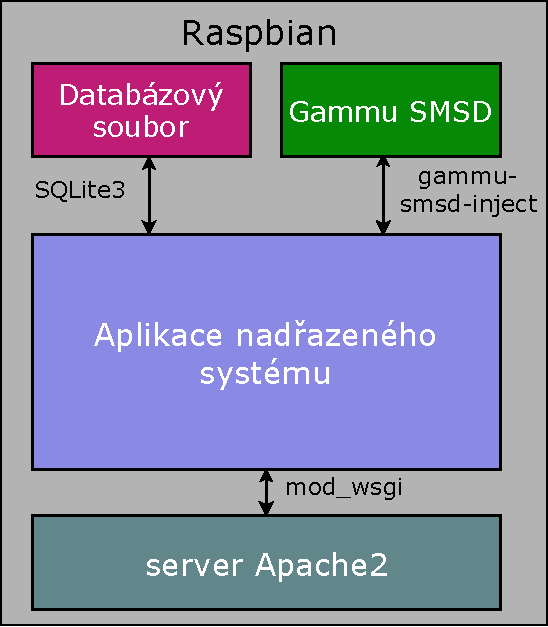
\includegraphics[width=0.8\textwidth]{images/sw_block.pdf}
    \caption[Softwarové blokové schéma nadřazeného systému]{Softwarové blokové schéma nadřazeného systému. Aplikace běží na OS Raspbian. Jako webový server je použit Apache2, se kterým aplikace komunikuje pomocí modulu mod\_wsgi \cite{mod_wsgi}. Databáze je upravována pomocí systému SQLite3, pro odesílání SMS s~upozorněními je použit program Gammu (bližší informace v~sekci \ref{sec:im_notifications}).}
    \label{fig:sw_block}
\end{figure}

V~této kapitole je stručně popsáno nasazení aplikace nadřazeného systému na jednodeskovém počítači Raspberry Pi 3 s~operačním systémem Raspbian. Blokové schéma nasazené aplikace je na obrázku \ref{fig:sw_block}. 

K~instalaci a spuštění aplikace je zapotřebí tento software:

\begin{itemize}
    \item Webový server Apache2.
    \begin{itemize}
        \item Nutno nainstalovat modul mod\_wsgi  \cite{mod_wsgi}.
    \end{itemize}
    \item Programovací jazyk Python3.
    \begin{itemize}
        \item Systém pro správu balíčků pip. Díky němu lze snado nainstalovat všechny potřebné Python moduly, jako například Flask nebo SQLAlchemy.
    \end{itemize}
    \item Program pro ovádání GSM modulu Gammu. Nadřazený systém je možné spustit i bez instalace tohoto programu, pouze nebude fungovat zasílání SMS upozornění.
\end{itemize}

\section{Konfigurace aplikace nadřazeného systému}
\label{sec:dp_appconfig}

Před nasazením aplikace je vhodné zvolit konfigurační soubor, který má být použit pro její nastavení. To je možné provést nastavením proměnné prostředí \texttt{GARAGE\_SYSTEM\_CONFIG} na cestu ke zvolenému souboru.

Pokud tato proměnná není nastavena, je použit výchozí konfigurační soubor \texttt{default\_config.py}.

\newpage

\section{Konfigurace Apache2}

Po instalaci potřebného softwaru je nejprve nutné nakonfigurovat server Apache2 tak, aby doručoval aplikaci nadřazeného systému. 

K~doručení Python aplikace je použit modul mod\_wsgi, jehož základní konfigurace je popsána v~článku \cite{flask_wsgi}. Spuštění aplikace pomocí mod\_wsgi je provedeno pomocí skriptu z~ukázky \ref{lst:wsgi_script}.

\begin{listing}[htbp]
\caption{\label{lst:wsgi_script} Skript pro spuštění aplikace na serveru Apache2 pomocí modulu mod\_wsgi. Skript importuje objekt aplikace nadřazeného systému (\texttt{app}), který je pak tímto modulem používán \cite{flask_wsgi}.}
\inputminted[bgcolor=codebg]{python}{source-samples/wsgi.py}
\end{listing}

\newpage

\subsection{Přístup k~databázi a souboru s~uživatelským nastavením}

Aplikace nadřazeného systému potřebuje měnit obsah databáze a souboru s~uživatelským nastavením (\texttt{user\_config.ini}). Je tedy nutné povolit uživateli, pod kterým aplikace běží, čtení a zápis těchto souborů. 

Apache2 spouští aplikace jako uživatel \texttt{www-data}, přístup k~souborům lze povolit způsobem popsaným v~ukázce \ref{lst:wwwdata}.

\begin{listing}[htbp]
\caption{\label{lst:wwwdata} Nastavení přistupových práv k~databázi a souboru s~uživatelským nastavením. Umístění souborů je možné nastavit v~konfiguračním souboru aplikace (viz sekci \ref{sec:dp_appconfig}).}
\inputminted[bgcolor=codebg]{bash}{source-samples/wwwdata.sh}
\end{listing}

\subsection{Konfigurace HTTPS}

Jelikož je při nasazení na Raspberry Pi použit \textit{self-signed} certifikát, vycházel jsem při konfiguraci HTTPS z~článku \textit{How To Create a Self-Signed SSL Certificate for Apache in Ubuntu 16.04} \cite{digital_ocean_selfsigned}.

Při konfiguraci HTTPS se ukázalo, že Apache2 nainstalovaný z~repozitářů Raspbianu nemá ve výchozím nastavení povolený SSL modul\footnote{Situace v~dubnu 2018.} a je nutné ho ručně povolit pomocí příkazu \texttt{a2enmod ssl}. Pro srovnání, při instalaci Apache2 na testovacím serveru ze sekce \ref{sec:te_deployment} byl tento modul povolen implicitně.

\section{Konfigurace Gammu SMSD}

Konfigurace démona Gammu SMSD je poměrně snadná, jak je vidět v~ukázce \ref{lst:gammurc}. Nejprve je potřeba zvolit způsob komunikace s~GSM modulem -- v~tomto případě jde o~AT příkazy (pro bližší informace viz \cite{gsm_standard}). Také je možnost nastavit explicitně rychlost sériové linky (například 19200 baudů).

Dále je třeba zvolit umístění zařízení. To nemusí být vždy \texttt{ttyUSB0}, konkrétní umístění lze zjistit po přípojení GSM modulu příkazem \texttt{dmesg | grep "GSM"}.

V~konfiguračním souboru je také zvoleno umístění složek, do kterých budou ukládány zprávy určené k~odeslání a již odeslané zprávy. Do složky zpráv k~odeslání (\texttt{outbox}) bude aplikace nadřazeného systému vkládat odesílaná upozornění pomocí příkazu \texttt{gammu-smsd-inject}. Je proto nutné, aby aplikace (respektive uživatel, pod kterým běží, což je \texttt{www-data}) měla přístup do této složky.

Při použítí výchozích složek (\texttt{/var/spool/gammu}), jako v~ukázce \ref{lst:gammurc}, stačí pro povolení přístupu přidat uživatele \texttt{www-data} do skupiny \texttt{gammu}. Tato skupina je vytvořena při instalaci programu Gammu.

\begin{listing}[htbp]
\caption{\label{lst:gammurc} Konfigurční soubor Gammu SMSD}
\inputminted[bgcolor=codebg]{ini}{source-samples/gammurc}
\end{listing}
